\subsection{Interface}

As interfaces fornecem uma maneira de definir contratos entre diferentes
classes, portanto, uma interface pode definir: a assinatura de métodos e
valores armazenados através de constantes. Por conta disto, qualquer classe  que
quiser seguir os padrões definidos pela interface deverá assinar um contrato,
ou seja, deverá implementar a assinatura dos métodos da mesma maneira como  fora
definido na interface \cite{programmingPhp}.

Além disto permite abstrair recursos em sistemas e facilitar a
injeção de dependências, além de garantir a extensibilidade e padronização do
projeto, ou seja, é possível definir que um objeto irá receber como argumento de
um método construtor uma interface, sendo que, é permitido passar como parâmetro
qualquer classe que implemente a interface.

Agora na Figura \ref{fig:interface} será apresentado um exemplo referente a
definição de uma interface utilizando a linguagem \acs{PHP}.

\begin{figure}[h!tb]
	\caption{Interface implementada na linguagem PHP}
	\label{fig:interface}

	\centering
	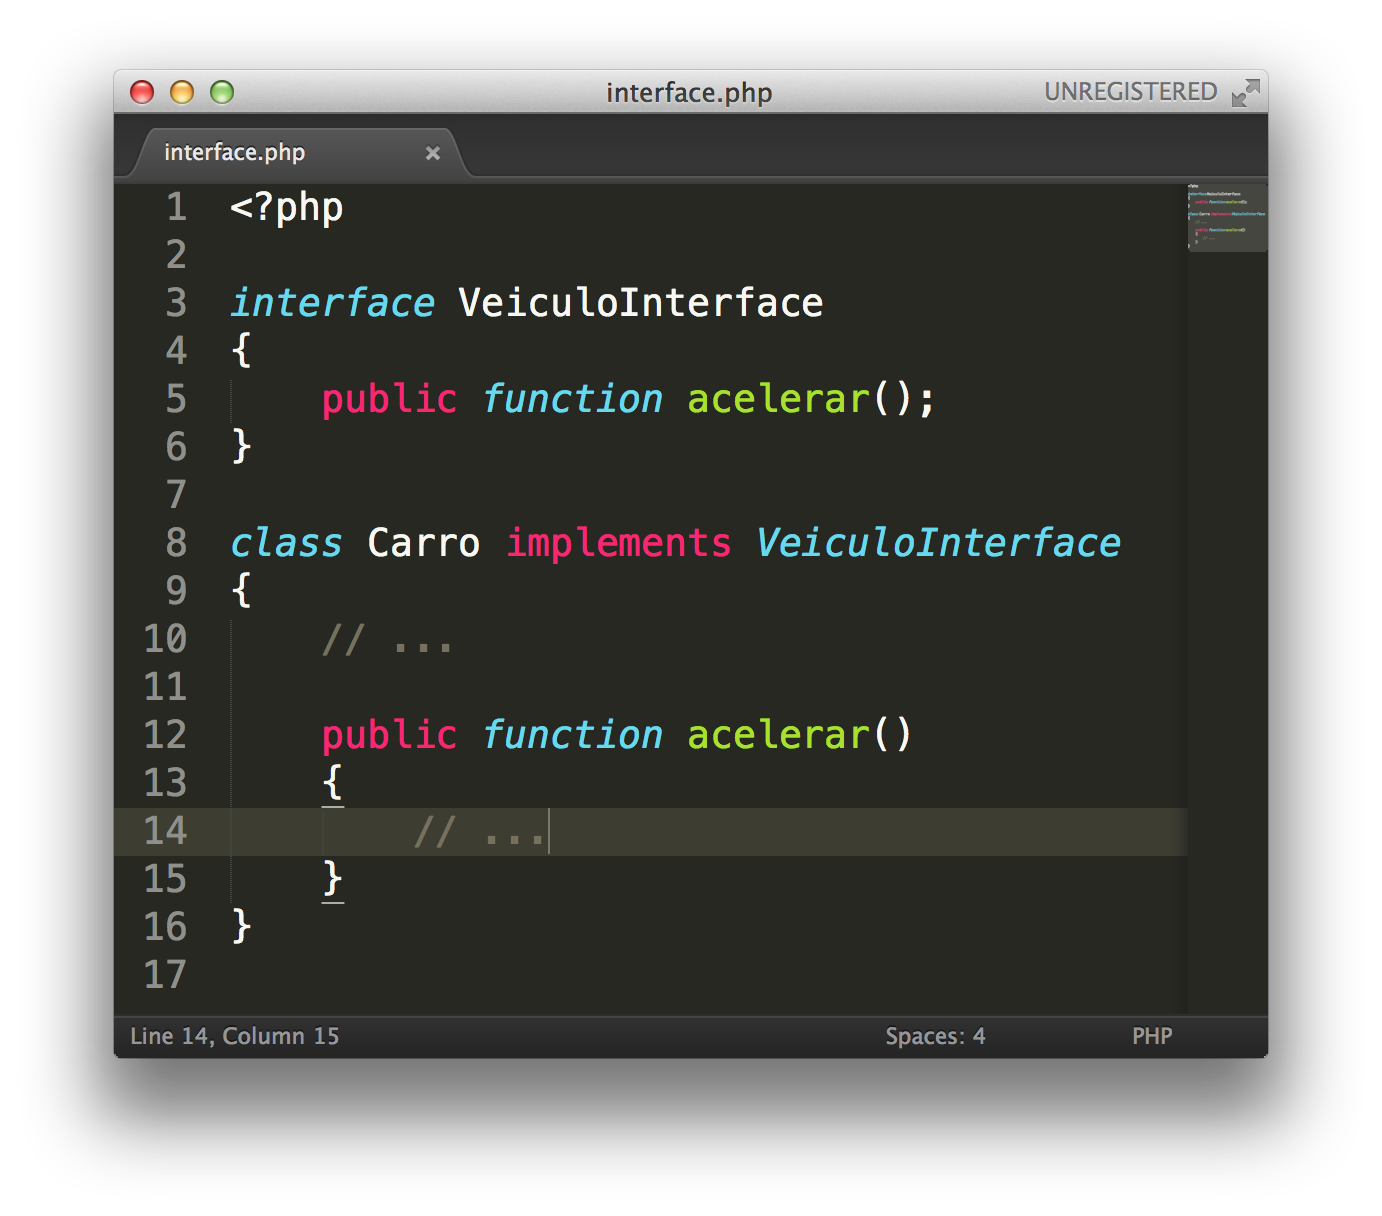
\includegraphics[width=0.75\textwidth]{images/interface.png}

	\centering
	\footnotesize Fonte: \fonteOAutor
\end{figure}

\FloatBarrier 	% Este comando impede que as imagens
				% flutuem a partir deste ponto no seu documento

A seguir, é apresentado em detalhes as linhas de código exibidas na Figura
\ref{fig:interface}:

\begin{alineas}
    \item linha 3: define-se uma interface nomeada como
    \textit{VeiculoInterface};
    \item linha 5: define-se a assinatura de um método, no qual, todas as
    classes que decidirem assinar um contrato com a interface deverão definir um
    método com a mesma assinatura;
    \item linha 8: implementa-se uma classe chamada \textit{Carro}, sendo que,
    ela assina um contrato com a interface \textit{VeiculoInterface}, por conta
    da palavra chave \textbf{implements};
    \item linha 12: define-se o método que foi solicitado pela interface.
\end{alineas}

Com isto, finaliza-se o capítulo que trata sobre os conceitos de orientação a
objetos com exemplos de implementação na linguagem \acs{PHP}, a seguir será
apresentado o capítulo que tratará sobre banco de dados.
